%!TeX root=../main.tex


% TODO:
%
% Figure cleanup:
%	- color correction on images
%	- spacing, layout, etc. of networks

\begin{figure}[!htb]   
\vskip -0.05in % useful knobs to optimize layout
    \centering        
    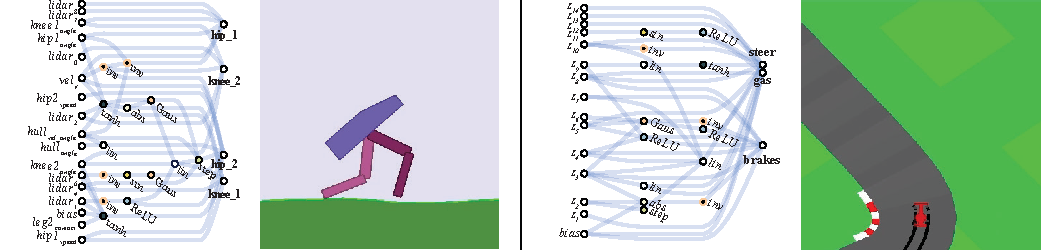
\includegraphics[width=1\textwidth]{img/cover.pdf}       
\vskip -0.05in % useful knobs to optimize layout
    \caption      
    {     
        \textit{Examples of Weight Agnostic Neural Networks: Bipedal Walker (left), Car Racing (right)}
        \newline
		We search for architectures by deemphasizing weights. In place of training, networks are assigned a single shared weight value at each rollout. Architectures that are optimized for expected performance over a wide range of weight values are still able to perform various tasks without weight training.
    }         
    \label{fig:cover_diagram} 
\vskip -0.05in % useful knobs to optimize layout
\end{figure}